
\chapter{Ondes électromagnétiques dans le vide}
\begin{tcolorbox}
\begin{figure}[H] %h:当前位置, t:顶部, b:底部, p:浮动页
  \centering
  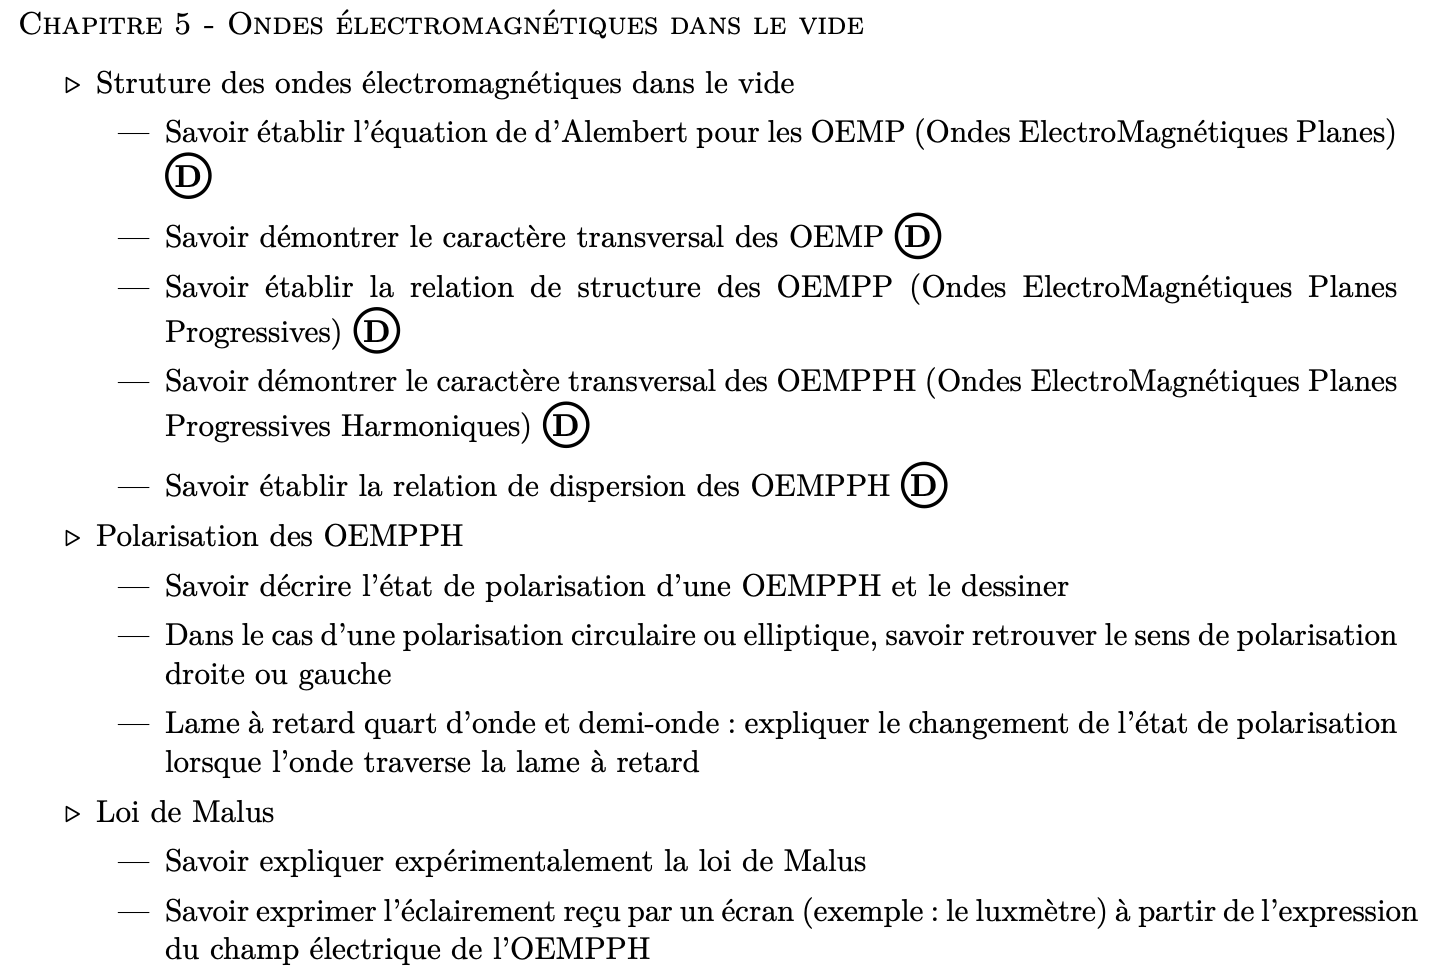
\includegraphics[width=\textwidth]{./assets/Programme du chapitre 5.png}
  \caption{Programme du chapitre 5}
  \label{fig:Programme du chapitre 5}
\end{figure}
\end{tcolorbox}


\newpage
\section{Structure des ondes électromagnétiques}

\subsection{Le champ électromagnétique dans le vide}
\label{sub:Le champ électromagnétique dans le vide}

Voir la partie 
\ref{sec:Champ électromagnétique dans le vide}

% subsection Le champ électromagnétique dans le vide (end)

\begin{Prop}{Champ Électromagnétique dans le vide}{}
Dans le vide,
\begin{itemize}
    \item Equation de Maxwell-Gauss (M.G.)
        \[
        \mathrm{div} \overrightarrow{E} (M,t) = 0
        \]
    \item Equation de Mawell-Flux (M.$\varphi$.)
        \[
        \mathrm{div} \overrightarrow{B} (M,t) = 0
        \]
    \item Equation de Maxwell-Faraday (M.F.)
        \[
        \overrightarrow{\mathrm{rot}}\overrightarrow{E} (M,t) = - \frac{\partial \overrightarrow{B} (M,t)}{\partial t}  
        \]
    \item Equation de Maxwell-Ampère (M.A.)
        \[
        \overrightarrow{\mathrm{rot} }  \overrightarrow{B} (M,t) = \varepsilon_0\mu_0 \frac{\partial \overrightarrow{E} (M,t)}{\partial t} 
        \]
\end{itemize}
\end{Prop}

\begin{Prop}{Équations de d'Alembert}{}
Les champs $\overrightarrow{E} (M,t)$ et $\overrightarrow{B} (M,t)$ peuvent être découplés, on obtient alors les équations de d'Alembert :
\begin{align*}
    \Delta \overrightarrow{E}  - \frac{1}{c^{2}} \frac{\partial ^{2}\overrightarrow{E} }{\partial t^{2}}  &= \overrightarrow{0} \\
    \Delta \overrightarrow{B}  - \frac{1}{c^{2}} \frac{\partial ^{2}\overrightarrow{B} }{\partial t^{2}}  &= \overrightarrow{0}
\end{align*}
\end{Prop}

\begin{myproof} Rappel que : $\overrightarrow{\mathrm{rot}}\overrightarrow{\mathrm{rot}}\overrightarrow{A} = \overrightarrow{\mathrm{grad}}\mathrm{div}\overrightarrow{A} - \Delta \overrightarrow{A}$
\begin{gather*}
    \overrightarrow{\mathrm{rot} } (\overrightarrow{\mathrm{rot} } \overrightarrow{E}) = \overrightarrow{\mathrm{rot} } \left( - \frac{\partial \overrightarrow{B} }{\partial t}  \right)  \\
\overrightarrow{\mathrm{grad} } \mathrm{div} \overrightarrow{E}  - \Delta \overrightarrow{E}  = - \frac{\partial }{\partial t} (\overrightarrow{\mathrm{rot} } \overrightarrow{B} )\\
-\Delta \overrightarrow{E}  = - \frac{\partial }{\partial t} \left( \varepsilon_0 \mu_0 \frac{\partial \overrightarrow{E} }{\partial t}  \right)  \\
    \Delta \overrightarrow{E}  - \frac{1}{c^{2}} \frac{\partial ^{2}\overrightarrow{E} }{\partial t^{2}}  = \overrightarrow{0}
\end{gather*}
On note $c^{2} = 1 / (\varepsilon_0 \mu_0)$, de même façon, on calcule le rotation de l'équation de (M.A)
\end{myproof}

\subsection{Ondes Electromagnétiques Planes}

\begin{Definition}[colbacktitle=red!75!black]{Onde électromagnétique plane (OEMP)}{}
    Un champ électromagnétique $\{ \overrightarrow{E} (M,t), \overrightarrow{B} (M,t)\}$ correspond à une \textbf{onde électromagnétique plane} dans la direction du vecteur unitaire $\overrightarrow{u}$, si :
    \begin{center}
    À chaque instant, $\overrightarrow{E} $ et $\overrightarrow{B} $ sont uniformes sur tout plan perpendiculaires à $\overrightarrow{u} $.
    \end{center}

    \begin{figure}[H] %h:当前位置, t:顶部, b:底部, p:浮动页
        \centering
        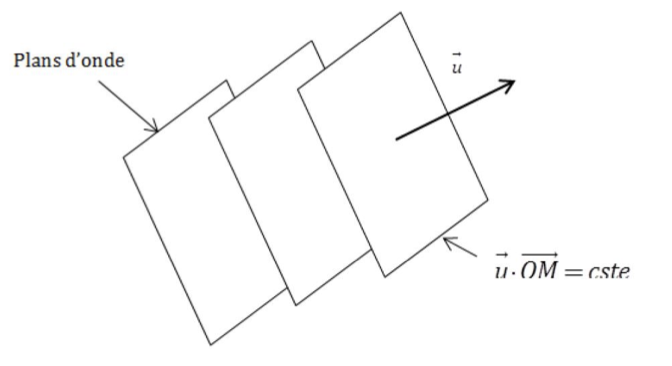
\includegraphics[width=0.5\textwidth]{./assets/Ondes Electromagnétiques Planes.png}
        \caption{Ondes Electromagnétiques Planes}
        \label{fig:Ondes-Electromagnétiques-Planes}
    \end{figure}

    \textbf{Plan d'ondes} : Les plans perpendiculaires à $\overrightarrow{u}$.
\end{Definition}

\begin{Prop}{Plan d'onde}{}
Les points $M$ appartenant à un plan perpendiculaire à $\overrightarrow{u}$ vérifie :
\[
  \overrightarrow{u}. \overrightarrow{OM} = C_{te}
\]

Les champes d'une OEMP s'écrivent sous la forme : $\overrightarrow{E} (\overrightarrow{u} .\overrightarrow{OM} ,t)$ et $\overrightarrow{B} (\overrightarrow{u} .\overrightarrow{OM} ,t)$, ou si on a choisit d'étudier des ondes planes dans la direction $\overrightarrow{e_z} $ par exemple, les champs s'écrivent $\overrightarrow{E} (z,t)$ et $\overrightarrow{B} (z,t)$
\end{Prop}


\begin{Prop}{Équation de d'Alembert unidimensionnelle}{}
\begin{itemize}
    \item On obtient l'\textbf{équation de d'Alembert unidimensionnelle} :
\[
\frac{\partial ^{2}\psi}{\partial z^{2}} (z,t) - \frac{1}{c^{2}} \frac{\partial ^{2}\psi}{\partial t^{2}} (z,t) = 0
\]
\item Les solutions générales sont de la forme :
\[
\psi(z,t) = f\left( t- \frac{z}{c}  \right)  + g\left( t + \frac{z}{c}  \right) 
\]

avec $f$ et $g$ correspondent respectivement à une onde progressive dans le sens des $z$ croissants et décroissants.

\item On peut remplacer :
  \[
    z \longleftrightarrow \overrightarrow{u}. \overrightarrow{OM}
  \]
    
\end{itemize}
\end{Prop}

\begin{Prop}{Vitesse de propagation}{}
Les ondes progreesives se propagent toutes à la vitesse : \textit{Indépendance du référentiel}
    \[
    c = \frac{1}{\sqrt{\varepsilon_0 \mu_0} } 
    \]
\end{Prop}



\begin{Prop}{Caractère transversal des OEMP}{}
    \center
    Les OEMP sont des ondes transversales
    \begin{figure}[H] %h:当前位置, t:顶部, b:底部, p:浮动页
      \centering
      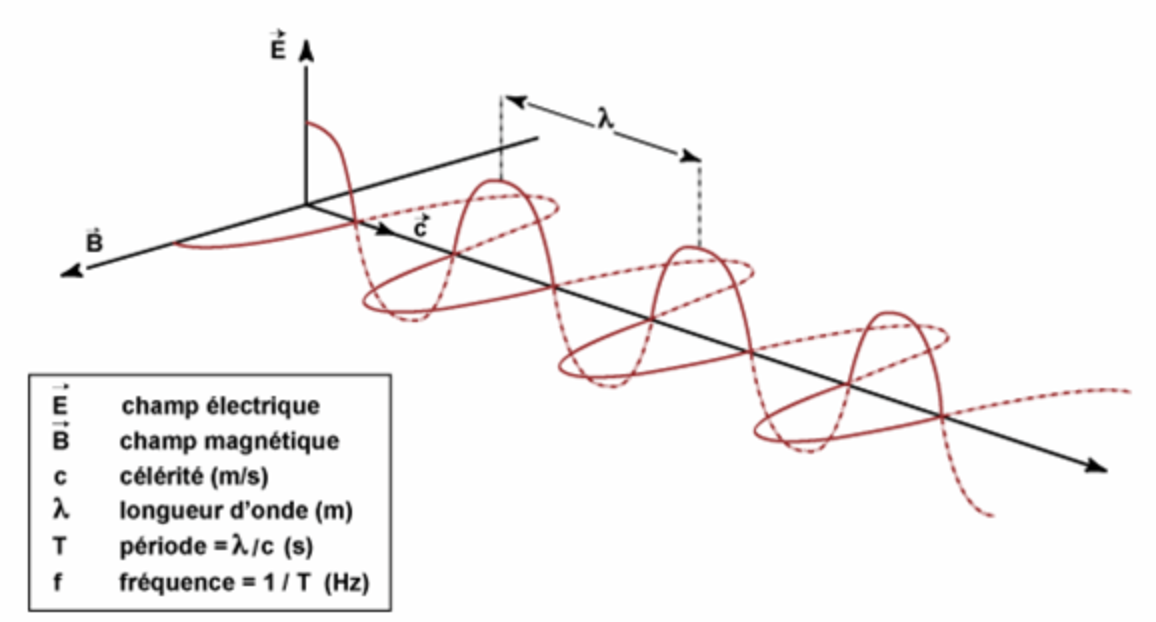
\includegraphics[width=0.5\textwidth]{./assets/Ondes Electromagnétiques Transversales.png}
      \caption{Ondes Electromagnétiques Transversales}
      \label{fig:${Ondes Electromagnétiques Transversales}}
    \end{figure}

            
        
\end{Prop}

\begin{myproof}
Supposons une onde plane dans la direction $\overrightarrow{u}  = \overrightarrow{e_z} $ 
\begin{itemize}
    \item D'abord, on a :
        \[
        \frac{\partial E_x}{\partial x} (z,t) = \frac{\partial E_y}{\partial y} (z,t) = 0
        \]
        
    \item (M.G.) donne 
        \[
        \mathrm{div} \overrightarrow{E}  = 0 \implies \frac{\partial E_z(z,t)}{\partial z} =0
        \]
        Conclusion : $E_z(t)$ ne dépend que du temps
    \item (M.A.) donne
        \[
          \overrightarrow{\mathrm{rot} }  \overrightarrow{B} (z,t) = \frac{1}{c^{2}}  \frac{\partial \overrightarrow{E} (z,t)}{\partial t} \implies \frac{\partial B_y(z,t)}{\partial x}  - \frac{\partial B_x(z,t)}{\partial y}  = \frac{1}{c^{2} }  \frac{\partial E_z(t)}{\partial t} \implies \frac{\partial E_z(t)}{\partial t} = 0
        \]
        Conclusion : $E_z$ est une vraie constante, composante uniforme
    \item Montrera par la suite que $E_z = 0$ et $B_z = 0$ (À revoir!)
\end{itemize}
\end{myproof}

\subsection{Ondes Electromagnétiques Planes Progressives}
On considère le cas d'ondes \textbf{progressives} dans la direction $\overrightarrow{e_z} $ : la fonction $f(t - z/c)$.

\begin{Prop}{Relation de structure}{}
\[
  \overrightarrow{B}  = \frac{1}{c} (\overrightarrow{e_z} \wedge \overrightarrow{E} \text{ ou } 
  \overrightarrow{B(M,t)}  = \frac{1}{c} (\overrightarrow{u} \wedge \overrightarrow{E}(M,t))
\]

\end{Prop}

\begin{myproof}
De la relation de Maxwell : 
\begin{gather*}
    \overrightarrow{\mathrm{rot}} \overrightarrow{B}  = \frac{1}{c^{2}} \frac{\partial \overrightarrow{E} }{\partial t} \iff \begin{bmatrix}
      0 \\ 0 \\ \frac{\partial }{\partial z} 
    \end{bmatrix}
    \wedge 
    \begin{bmatrix}
      B_x \\ B_y \\ 0
    \end{bmatrix}
    = 
    \frac{1}{c ^2} \frac{\partial }{\partial t} \begin{bmatrix}
      E_x \\E_y\\0
    \end{bmatrix} \\
    - \frac{\partial B_y}{\partial z}  = \frac{1}{c^{2}}  \frac{\partial E_x}{\partial t}  \text{ et } \frac{\partial B_x}{\partial z}  = \frac{1}{c^{2}}  \frac{\partial E_y}{\partial t}
\end{gather*}

La relation entre les dérivées démontre que, pour $f(t-z/c)$, 
\[
  \frac{\partial f}{\partial z } = - \frac{1}{c} \frac{\partial f }{\partial t}  
\]
Donc, 
\[
    \frac{1}{c} \frac{\partial B_y}{\partial t} = \frac{1}{c^{2}} \frac{\partial E_x}{\partial t} = - \frac{1}{c^{2}} \frac{\partial E_y}{\partial t}
\]
D'où en considérant les constantes d'intégration nulles : $B_y = \frac{1}{c} E_x$ et $B_x = -\frac{1}{c} E_y$.
\end{myproof}

\subsection{Aspects énergétiques de l'OEMPP dans le vide}
Voir chapitre 2 - Aspects énergétiques de l'électromagnétisme

\newpage
\section{Ondes Electromagnétiques Planes Progressives Harmoniques}

\subsection{Définitions}
\begin{Definition}[colbacktitle=red!75!black]{Onde plane progressive harmonique (OEMPPH)}{}
En physique ondulatoire, une onde progressive harmonique est sous la forme :
\[
\psi(M,t) = A \cos ( \omega t - \overrightarrow{k} .\overrightarrow{OM} + \varphi)
\]

où
\begin{itemize}
    \item $ \omega $ la \textbf{pulsation de l'onde}
    \item $\overrightarrow{k}$ le \textbf{vecteur d'onde}
    \item $\varphi$ la \textbf{phase} de l'onde à l'origine
    \item $A$ l'\textbf{amplitude} de la grandeur $\varphi$
\end{itemize}

Par exemple, nous écrirons les composantes du champ $\overrightarrow{E} $ sous la forme :
\[
E_i = E_{i_0} \cos( \omega t - \overrightarrow{k} . \overrightarrow{OM} + \varphi_{E_i})
\]

On introduit le vecteur unitaire parallèle à $\overrightarrow{k} $ :
\[
\overrightarrow{u}  = \frac{\overrightarrow{k} }{ \|\overrightarrow{k}\|  } 
\]
\end{Definition}

\begin{Prop}{Double périodicité}{}
  \begin{itemize}
    \item Périodicité temporelle : $T$ 
    \item Périodicité spatiale, appelée \textbf{longueur d'onde} : $\lambda$
    \item \textbf{Pulsation spatiale} : $k$
  \end{itemize}

\[
  T = \frac{2\pi}{\omega}, \; \lambda = \frac{2\pi}{k} \text{ avec } k = \| \overrightarrow{k} \|
\]
\end{Prop}

\begin{Prop}{Vitesse de phase d'une OEMPPH }{}
\[
v_\varphi = \frac{\omega}{k} 
\]
\end{Prop}
\begin{myproof}{}{}
\[
  \psi (z,t) = A \cos(\omega t - kz + \varphi) = A \cos \left( \omega \left( t - \frac{z}{(\omega/k)}\right)+ \varphi\right) = \psi \left( 0, t - \frac{z}{\omega/k}\right)
\]
\end{myproof}


\begin{Prop}{Représentation complexe d'une OEMPPH}{}
En notation complexe, $\overrightarrow{E}  = \mathrm{Re} (\overrightarrow{\underline{E}} )$, et $\overrightarrow{B} = \mathrm{Re} (\overrightarrow{\underline{B}}) $, on généralise :
\[
    \overrightarrow{\underline{E}}  = \overrightarrow{\underline{E_0}} \exp [j( \omega t - \overrightarrow{k} .\overrightarrow{OM} )],\;
    \overrightarrow{\underline{B}}  = \overrightarrow{\underline{B_0}} \exp [j( \omega t - \overrightarrow{k} .\overrightarrow{OM} )] 
\]
\end{Prop}

\begin{Prop}{Opérateurs en représentation complexe}{}
Remplace 
\[
  \overrightarrow{\nabla } \longleftrightarrow -j\overrightarrow{k}, \; \frac{\partial }{\partial t} \to j \omega
\]
On aura aussi: 
\[
    \overrightarrow{\mathrm{rot} } \overrightarrow{\underline{E}}  = -j \overrightarrow{k} \wedge \overrightarrow{\underline{E}} , \quad \mathrm{div} \overrightarrow{\underline{E}} = -j \overrightarrow{k} . \overrightarrow{\underline{E}} , \quad \frac{\partial \overrightarrow{\underline{E}} }{\partial t}  = j \omega \overrightarrow{\underline{E}} , \quad \Delta \overrightarrow{E}  = - k^{2}\overrightarrow{E}
\]
\end{Prop}

\begin{myproof}{}{}
Rappel :
\[
\overrightarrow{\nabla }  = \begin{bmatrix} \frac{\partial }{\partial x} \\ \frac{\partial }{\partial y} \\ \frac{\partial }{\partial z}  \end{bmatrix}
\]
\end{myproof}


\subsection{Relation de dispersion}

\begin{Prop}{Relation de dispersion des OEMPPH dans le vide}{}
\[
\omega = ck,\quad \lambda = c\times T
\]

Pour les OEMPPH, la vitesse de phase est la vitesse de lumière :
\[
  v_\varphi = \frac{ \omega }{k} =c
\]

\end{Prop}
\begin{myproof}
En représentation complexe, 
\begin{gather*}
    \Delta \overrightarrow{E}  - \frac{1}{c^{2}}  \frac{\partial ^{2}\overrightarrow{E} }{\partial t ^{2}}  = \overrightarrow{0}  \implies \left( -k^{2}+ \frac{ \omega ^{2}}{c^{2}}  \right) \times \overrightarrow{\underline{E}}  = \overrightarrow{0} \\
    k^{2} = \frac{ \omega ^{2}}{c^{2}}  \implies k = \pm \frac{\omega}{c} (\text{OPPH+, OPPH}-)
\end{gather*}
\end{myproof}

\subsection{Polarisation des OEMPPH}
\begin{Definition}[colbacktitle=red!75!black]{Direction de polarisation de l'onde}{}
La \textit{direction du vecteur champ} $\overrightarrow{E} $ d'une OEMPPH détermine la direction de \textbf{polarisation de l'onde}.

La direction du champ $\overrightarrow{B} $ se déduit de celle de $\overrightarrow{E} $ car $(\overrightarrow{u} , \overrightarrow{E} ,\overrightarrow{B} )$ est une base directe.
\end{Definition}

\begin{Prop}{Cas général : OEMPPH polarisée elliptiquement}{}
Pour $\overrightarrow{k} = k\overrightarrow{e_z}$ (avec $k>0$), les composantes du champ $\overrightarrow{E} $ d'une OEMPPH sont, avec $E_{0x}$, $E_{0y}$ positifs :
\[
    \overrightarrow{E} (M,t) = \begin{bmatrix} E_{0x}\cos ( \omega t'- kz + \varphi_x) \\E_{0y}\cos ( \omega t'- kz + \varphi_y)\\ 0 \end{bmatrix} 
\]

En changeant l'origine des temps et en se plaçant en $z=0$, on a :
\[
    \overrightarrow{E} (M,t) = \begin{bmatrix} E_{0x}\cos ( \omega t'- kz ) \\E_{0y}\cos ( \omega t'- kz + \varphi)\\ 0 \end{bmatrix} \text{ avec } \varphi = \varphi_y - \varphi_x
\]


À $z$ fixé, l'éxtrémité de $\overrightarrow{E}$ parcourt une ellipse dans le plan $\{\overrightarrow{e_x} , \overrightarrow{e_y} \}$. On parle de \textbf{polarisation elliptique}.

\[
\tan 2 \alpha  = \frac{2E_{0x}E_{0y}}{E_{0x}^{2} - E_{0y}^{2}} \cos \varphi 
\]

\begin{figure}[H] %h:当前位置, t:顶部, b:底部, p:浮动页
    \centering
    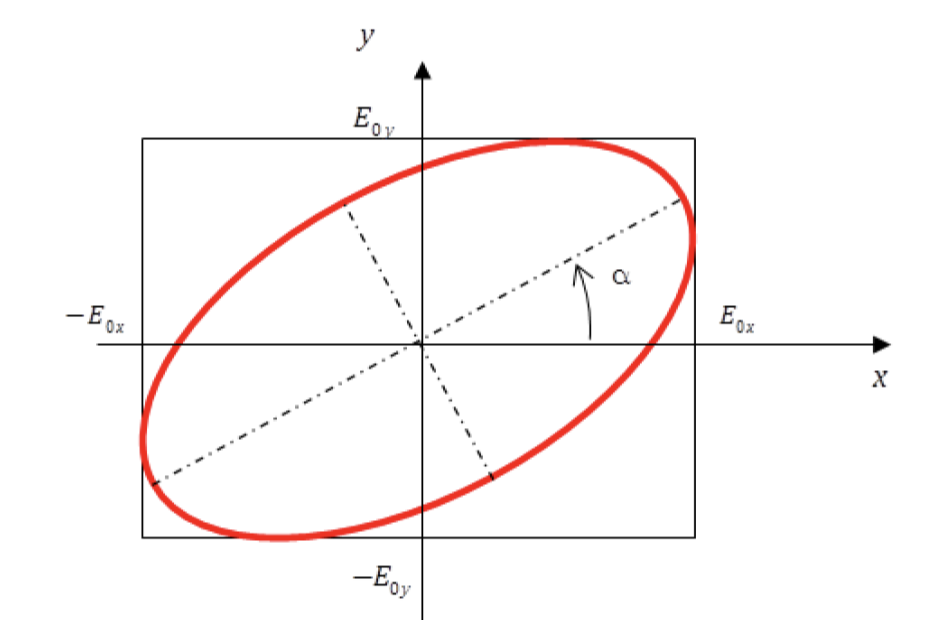
\includegraphics[width=0.5\textwidth]{./assets/Polarisation Ellipse.png}
    \caption{Polarisation Ellipse}
    \label{fig:Polarisation-Ellipse}
\end{figure}
Le sens de parcours dépend du signe de $\varphi$,  $\varphi>0$ en  \textbf{avance} sinon en \textbf{retard}. $\varphi >0$ tourne en sens droite.



\end{Prop}

\begin{myproof}
Équation d'un conique : $ax^{2}+2bxy+cy^{2}+2dx+2ey+f=0$ avec $x = E_x$, $y=E_y$, c'est un éllipse si $ac-b^{2}<0$.

\begin{gather*}
    E_x = E_{0 x} \cos ( \omega t) \implies \frac{E_x}{E_0x}  = \cos( \omega t) \\
    E_y = E_{0y} \cos ( \omega t+\varphi) = E_0y [\cos \omega t \cos \varphi - \sin \omega t \sin \varphi] \implies \sin (\omega t) \sin \varphi = \frac{E_x}{E_{0x}} \cos \varphi - \frac{E_y}{E_{0y}}  
\end{gather*}

Comme $\cos^{2} \omega t+ \sin ^{2} \omega t = 1$,
\begin{gather*}
    \left( \frac{E_x}{E_{0x}}  \right) ^{2}  + \left( \frac{E_x}{E_{0x}} \left( \frac{\cos \varphi}{\sin \varphi}  \right)- \frac{E_y}{E_{0y}} \frac{1}{\sin \varphi}    \right) ^{2} = 1 \\
    \left( \frac{E_x}{E_{0x}}  \right) ^{2} \sin ^{2} \varphi + \left( \frac{E_x}{E_{0x}}  \right) ^{2} \cos^{2}\varphi + \left( \frac{E_y}{E_{0y}}  \right) ^{2} - 2 \left( \frac{E_x}{E_{0x}}  \right)  \cos \varphi \left( \frac{E_y}{E_{0y}}  \right)  = \sin ^{2}\varphi \\
    \left( \frac{E_x}{E_{0x}}  \right) ^{2} + \left( \frac{E_y}{E_{0y}}  \right)  ^{2} - 2 \left( \frac{E_x}{E_{0x}}  \right) \left( \frac{E_y}{E_{0y}}  \right)  \cos \varphi - \sin ^{2} \varphi=0
\end{gather*}

Dans la forme $ax^{2}+cy^{2}+ 2bxy+2dx+2ey+f = 0$, $a=1$,  $c=1$,  $b = -\cos \varphi$,  $d=0$,  $e=0$,  $f = - \sin ^{2}\varphi$.


Ellipse si $ac-b^{2}>0$ et $1\times 1 - (-\cos \varphi)^{2} >0$

\end{myproof}

\begin{figure}[H] %h:当前位置, t:顶部, b:底部, p:浮动页
    \centering
    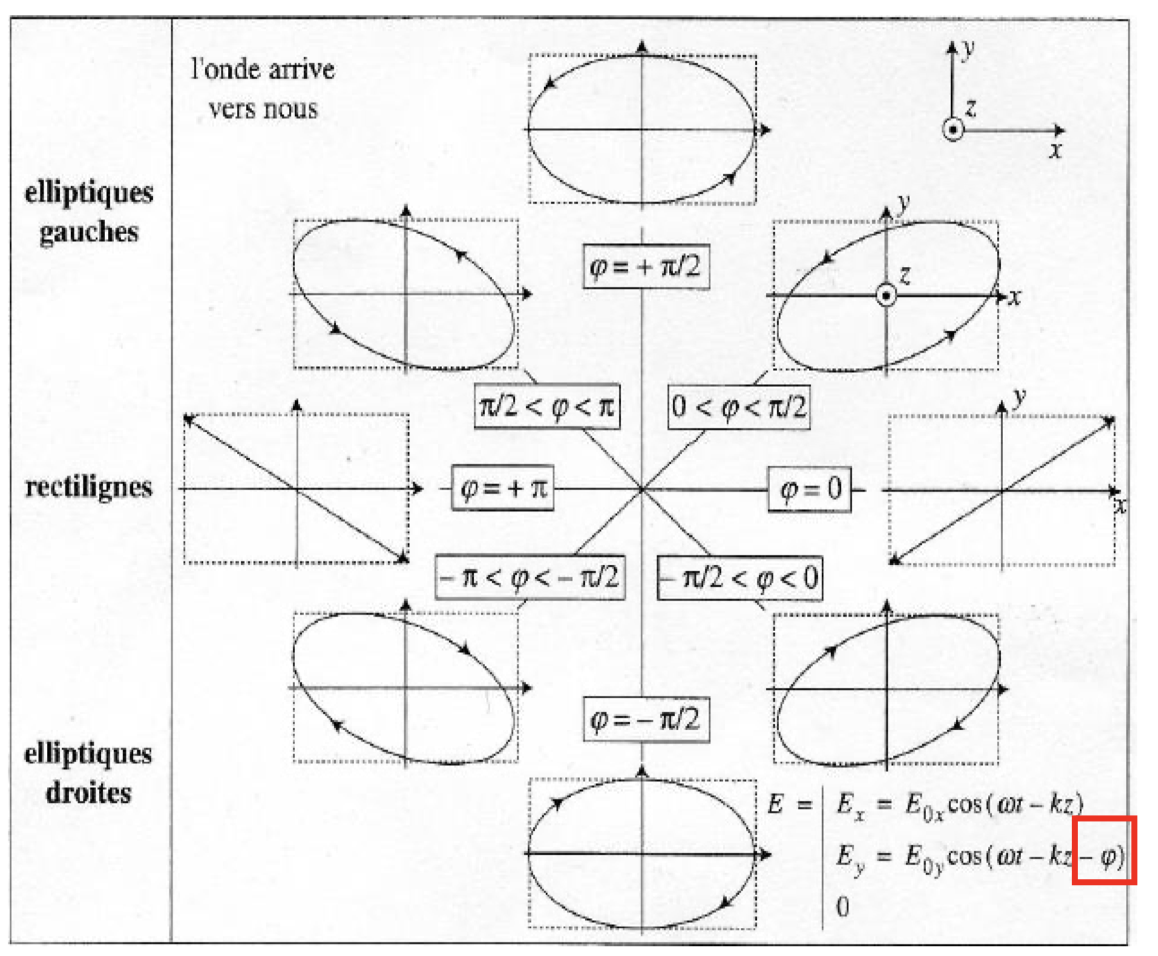
\includegraphics[width=0.5\textwidth]{./assets/Sens de polarisation.png}
    \caption{Sens de polarisation (Importante de savoir, ce résumé dépend de la convention observateur, la signe de $\varphi$ peut changer)}
    \label{fig:Sens-de-polarisation}
\end{figure}

\begin{Prop}{Polarisation rectiligne}{}
Le vecteur champ $\overrightarrow{E}$ grade une direction fixe dans l'espace, on parle de  \textbf{polarisation rectiligne}.

C'est lorsque le cas où $\varphi=0$ et $\varphi = \pi$
\end{Prop}

\begin{myproof} Comme $E_x = E_{0x} \cos \omega t$ et $E_y = E_{0y} \cos \omega t$ ou $E_y = E_{0y} \cos (\omega t + \pi)$
\begin{gather*}
    \frac{E_x}{E_y}  = \frac{E_{0x}}{E_{0y}}  \implies E_y = \left( \frac{E_{0y}}{E_{0x}}  \right) E_x \\
    \frac{E_x}{E_y}  = -\frac{E_{0x}}{E_{0y}}  \implies E_y = -\left( \frac{E_{0y}}{E_{0x}}  \right) E_x
\end{gather*}
On obtient une droite sous la forme $y=ax+b$ et $y = -ax+b$ ($b=0$) 
\end{myproof}

\begin{Prop}{Polarisation circulaire}{}
Cas particulier où $E_{0x} = E_{0y } = E_0$ et $\varphi = \pm \pi / 2$
\end{Prop}

\begin{myproof}
Sachant que $E_x = E_0 \cos \omega t$ et $E_y = \pm E_0 \sin \omega t$,
\begin{gather*}
\cos ^{2} \omega t + \sin ^{2} \omega t = 1 \implies \left( \frac{E_x}{E_0}  \right)  ^{2} + \left( \pm \frac{E_y}{E_0}  \right)  ^{2} = 1
\end{gather*}
\end{myproof}

Une OEMPPH est décompsable en somme de deux ondes polarisées \textit{rectilignement} dans des directions perpendiculaires.

\[
\overrightarrow{E}  = \exp(j( \omega t - kz) )\begin{cases}
    E_{0x} \\ E_{0y} \exp(j\varphi) 
\end{cases} = \exp (j ( \omega t - kz)) \begin{cases}
    E_{0x} \\ 0 
\end{cases} + \exp (j ( \omega t - kz)) \begin{cases}
    0 \\ E_{0y} \exp(j \varphi)
\end{cases}
\]

Une OEMPPH est décomposable en un somme de deux ondes polarisées \textit{circulairement} dans deux sens opposés.

\[
\overrightarrow{E}  = \exp (j( \omega t-kz)) \times  \left( \frac{E_{0x} - jE_{0y} \exp(j\varphi)}{2}  \right)  \times  \begin{cases}
    1 \\ j
\end{cases} + \exp (j( \omega t - kz)) \times  \left( \frac{E_{0x}+ j E_{0y} \exp (j\varphi)}{2}  \right)  \times \begin{cases}
    1 \\ -j
\end{cases}
\]




\newpage
\section{La lumière comme onde électromagnétique}

\subsection{Signal Lumineux} % (fold)
\label{sub:Signal Lumineux}

% subsection Signal Lumineux (end)

Dans l'optique ondulatoire et le signal lumineux :
\[
  \boxed{I = 2 \langle  s^{2}(M,t)  \rangle \iff \mathcal{E}  = K \langle  E^{2}(M,t)  \rangle } = \frac{1}{2c \mu_0}  (E_{0x}^{2} + E_{0y}^{2})
\]


\begin{itemize}
    \item $\mathcal{E}$ : Eclairement (unité : lux $\mathrm{lx}$), mesuré avec un luxmètre
    \item $I$ : Intensité lumineuse
    \item $K$ : constante qui dépend du capteur et de constantes
\end{itemize}

\subsection{Polarisation de la lumière} % (fold)
\label{sub:Polarisation de la lumière}

\begin{Prop}{Lumière Naturelle}{}
La plupart des sources lumineuses naturelles délivrent 
\begin{itemize}

    \item des ondes \underline{non polarisées}
    \item des trains d'ondes \underline{incohérentes}

\end{itemize}
\end{Prop}

\begin{Definition}[colbacktitle=red!75!black]{Polariseurs}{}
  \begin{figure}[H] %h:当前位置, t:顶部, b:底部, p:浮动页
    \centering
    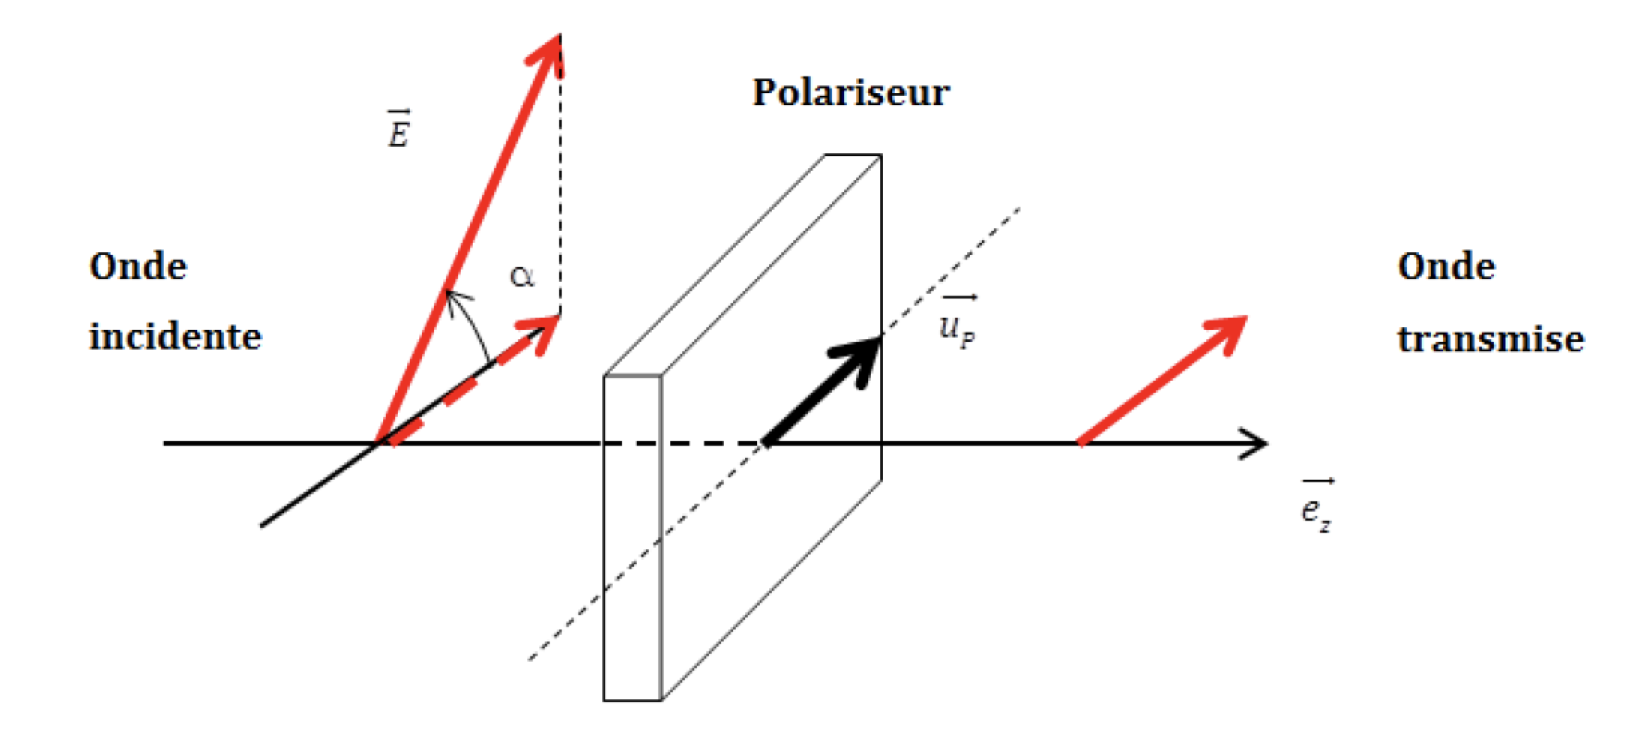
\includegraphics[width=0.8\textwidth]{./assets/Polariseur rectiligne.png}
    \caption{Polariseur rectiligne}
  \end{figure}

  
Un \textbf{polariseur} idéal possède une direction liée au système, de vecteur directeur $\overrightarrow{u_p}$, telle que : 
\begin{itemize}

    \item Tout onde polarisée rectilignement \underline{perpendiculairement à} $\overrightarrow{u_p}$ est \underline{totalement absorbée}
    \item Tout onde polarisée rectilignement \underline{parallèlment à} $\overrightarrow{u_p}$ est \underline{totalement transmise}

\end{itemize}
\end{Definition}






% subsection Lois de Malus (end)

% subsection Polarisation de la lumière (end)

\begin{Definition}[colbacktitle=red!75!black]{Lame à retard de phase}{}
\textbf{Lames à retard} : Une lame à retard de phase est un crital \textit{biréfringent} capable de modifier la polarisation de la lumière la traversant.

\textbf{Axe rapide}, \textbf{axe lent} : On note respectivement $n_L$, $n_R$ d'axes lent ou rapide. 

\center 
Comme $v = c / n$, Si $v_y< v_x$, donc $n_L > n_R$.

\begin{figure}[H] %h:当前位置, t:顶部, b:底部, p:浮动页
  \centering
  \includegraphics[width=0.5\textwidth]{./assets/Lame à retard de phase.png}
  \caption{Lame à retard de phase}
  \label{fig:Lame à retard de phase}
\end{figure}


\end{Definition}



\begin{Prop}{}{} 
  Dans la figure \ref{fig:Lame à retard de phase}, la composante $E_y$ du champ incident prend un \underline{retard} de phase par rapport à $E_x$ d'une valeur de : 
\begin{equation}
  \Delta \varphi = \frac{2 \pi}{\lambda_0}  (n_L - n_R)e >0
\end{equation}
Avant la traversée de la lame $\implies$ Après la traversée de la lame :
\begin{equation}
  \overrightarrow{E} = \begin{cases} 
    E _{0x}  \cos ( \omega t - kz) \\ 
    E _{0y} \cos ( \omega t - kz + \varphi) \\ 
    0
  \end{cases} \implies 
  \overrightarrow{E'} = \begin{cases}
    E' _{0x}  \cos ( \omega t - kz) \quad\quad\quad\text{rapide}\\ 
    E' _{0y} \cos ( \omega t - kz + \varphi - \Delta \varphi) \quad\text{lent}\\ 
    0
  \end{cases}
\end{equation}

avec $\Delta \varphi = k_0 \delta = \frac{2 \pi}{\lambda_0} \times \Delta n \times e$. 
\end{Prop}

\begin{Definition}[colbacktitle=red!75!black]{Lame $\lambda/2$ et $\lambda/4$}{}
  \begin{itemize}

      \item Lame $\lambda/2$ : $\Delta n \times e = \lambda/2 \implies \Delta \varphi = \pm \pi$
      \item Lame $\lambda/4$ : $\Delta n \times e = \lambda/4 \implies \Delta \varphi = \pm \pi/2$

  \end{itemize}
\end{Definition}

\begin{figure}[H] %h:当前位置, t:顶部, b:底部, p:浮动页
  \centering
  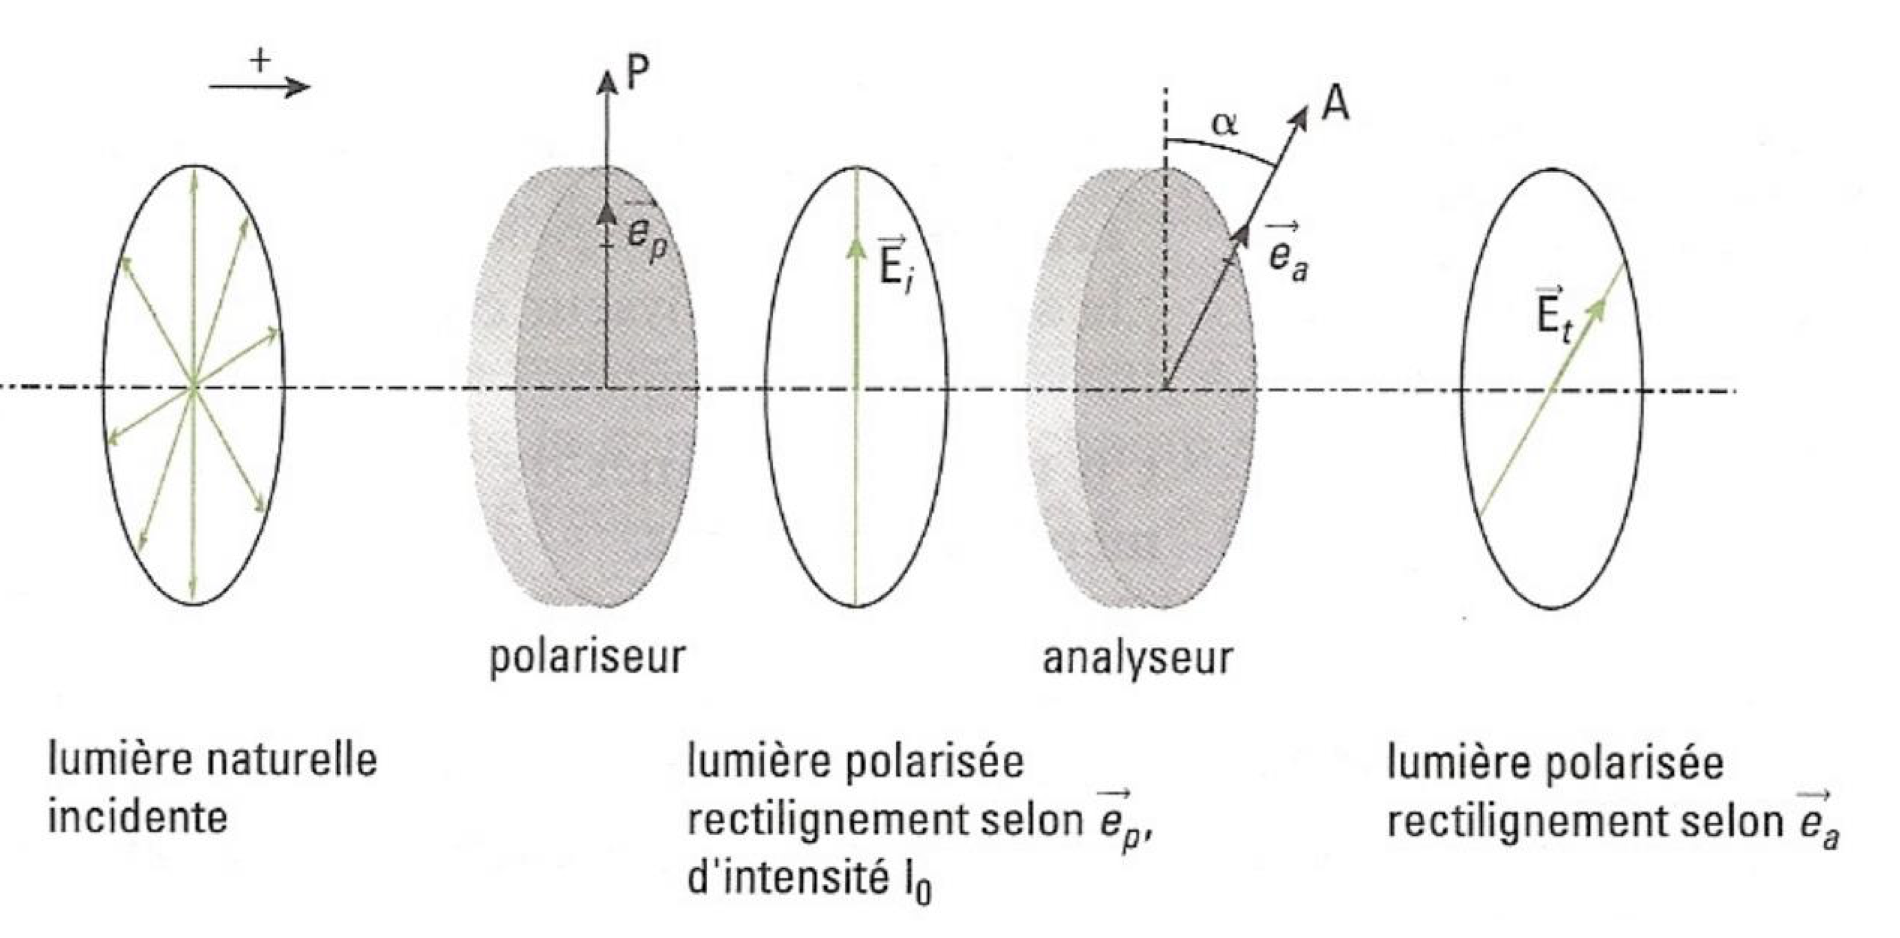
\includegraphics[width=0.8\textwidth]{./assets/Polariseur + Analyseur.png}
  \caption{Polariseur + Analyseur}
  \label{fig:Polariseur + Analyseur}
\end{figure}

\begin{figure}[H] %h:当前位置, t:顶部, b:底部, p:浮动页
  \centering
  \includegraphics[width=0.8\textwidth]{./assets/Dispositif Expérimental.png}
  \caption{Dispositif Expérimental}
  \label{fig:Dispositif Expérimental}
\end{figure}

\begin{Example}{Polarisation à la sortie (Cas $\lambda/2$)}{}
  \begin{itemize}

      \item Positionner les deux polariseurs en position croisée pour obtenir l’\underline{extinction}.
      \item Placer une lame demi-onde entre les deux polariseurs. Relever les directions des lignes neutres de la lame. 
\item Tourner la lame de 25° par rapport à l’une des lignes neutres.

  \end{itemize}
\begin{figure}[H] %h:当前位置, t:顶部, b:底部, p:浮动页
  \centering
  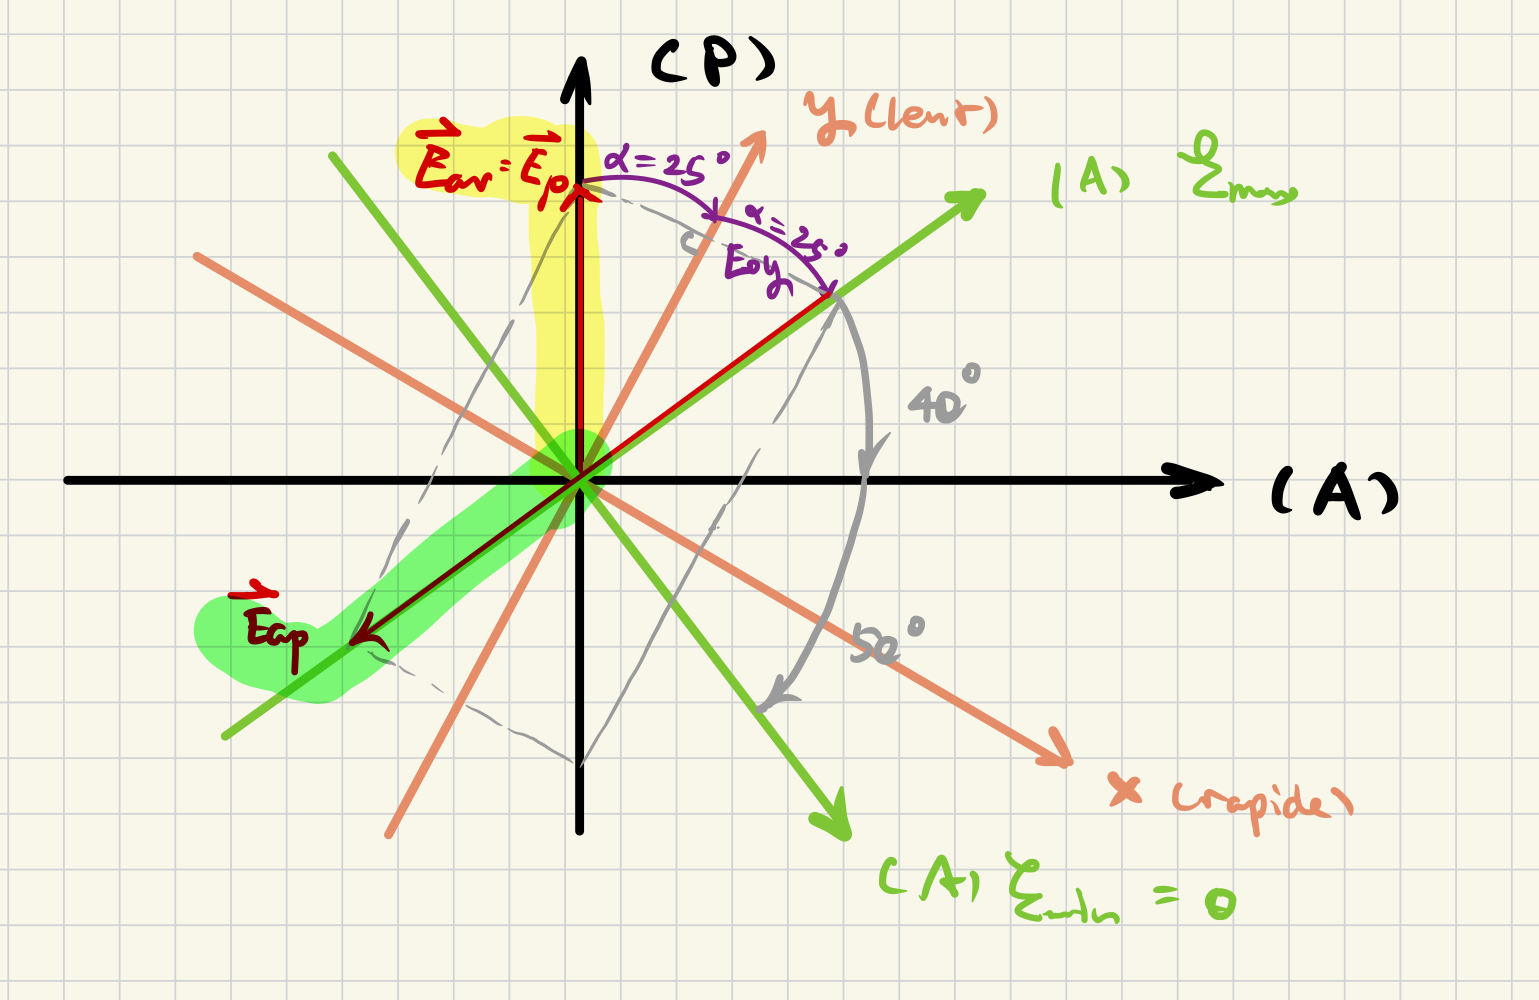
\includegraphics[width=0.6\textwidth]{./assets/Lame demi-onde.jpeg}
  \caption{Lame demi-onde $\lambda/2$}
\end{figure}

$\overrightarrow{E_p} = E_p . \overrightarrow{u_p}$ avec $E_p = E_0 \cos \omega t$

\begin{equation}
  \overrightarrow{E} _{av} = \begin{cases}
    - E_0 \sin \alpha \cos \omega t \\ 
    E_0 \cos \alpha \cos \omega t \\ 
    0
  \end{cases} \implies 
  \overrightarrow{E} _{ap} = \begin{cases}
    - E_0 \sin \alpha \cos \omega t \\ 
    E_0 \cos \alpha  \cos (\omega t - \pi)  = - E_0 \cos \alpha \cos \omega t\\ 
    0
  \end{cases}
\end{equation}

Conclusion : Symétrie selon l'axe rapide, et $(A)$ a tourné de $2 \alpha$ dans le même sens que $\lambda/ 2$.
\end{Example}

\begin{Example}{Polarisation à la sortie (Cas $\lambda/4$)}{}
  \begin{itemize}

      \item Positionner les deux polariseurs en position croisée pour obtenir l’extinction.
      \item Placer une lame quart d’onde entre les deux polariseurs. Relever les directions des lignes neutres de la lame.

  \end{itemize}
  Trouver une onde plane progressive monochromatique de polarisation circulaire :
\begin{figure}[H] %h:当前位置, t:顶部, b:底部, p:浮动页
  \centering
  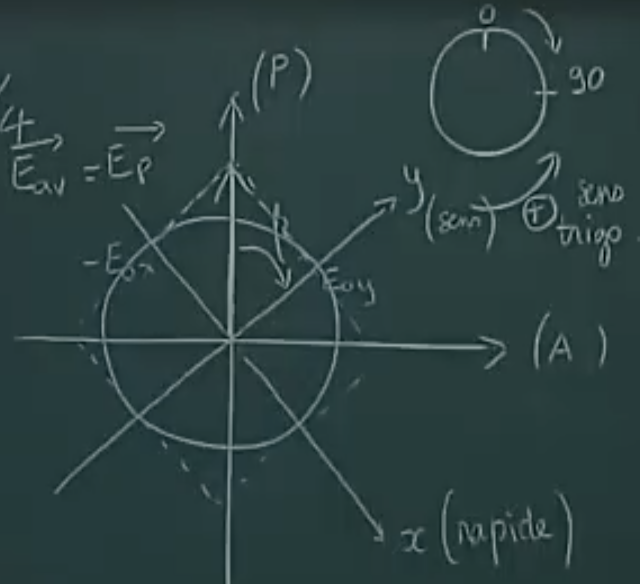
\includegraphics[width=0.5\textwidth]{./assets/Lame quart d'onde.png}
  \caption{Lame quart d'onde}
  \label{fig:Lame quart d'onde}
\end{figure}

$\overrightarrow{E_p} = E_p .\overrightarrow{u_p} = \overrightarrow{E} _{av}$ 

\begin{equation}
  \overrightarrow{E} _{av} = \begin{cases}
    - E_0 \sin \alpha \cos \omega t \\ 
    E_0 \cos \alpha \cos \omega t \\ 
    0
  \end{cases} \implies 
  \overrightarrow{E} _{ap} = \begin{cases}
    - E_0 \sin \alpha \cos \omega t \\ 
    E_0 \cos \alpha  \cos \left(\omega t - \frac{\pi}{2} \right)  = - E_0 \cos \alpha \sin \omega t\\ 
    0
  \end{cases}
\end{equation}

\end{Example}
Conclusion : Il faut $E_0 \sin \beta = E_0 \cos \beta$ donc $\beta = \pi /4 = 45 ^{\circ}$

\begin{Example}{Application : PCG}{}
\textbf{PCG} : produire une OEMPPM.

\begin{figure}[H] %h:当前位置, t:顶部, b:底部, p:浮动页
  \centering
  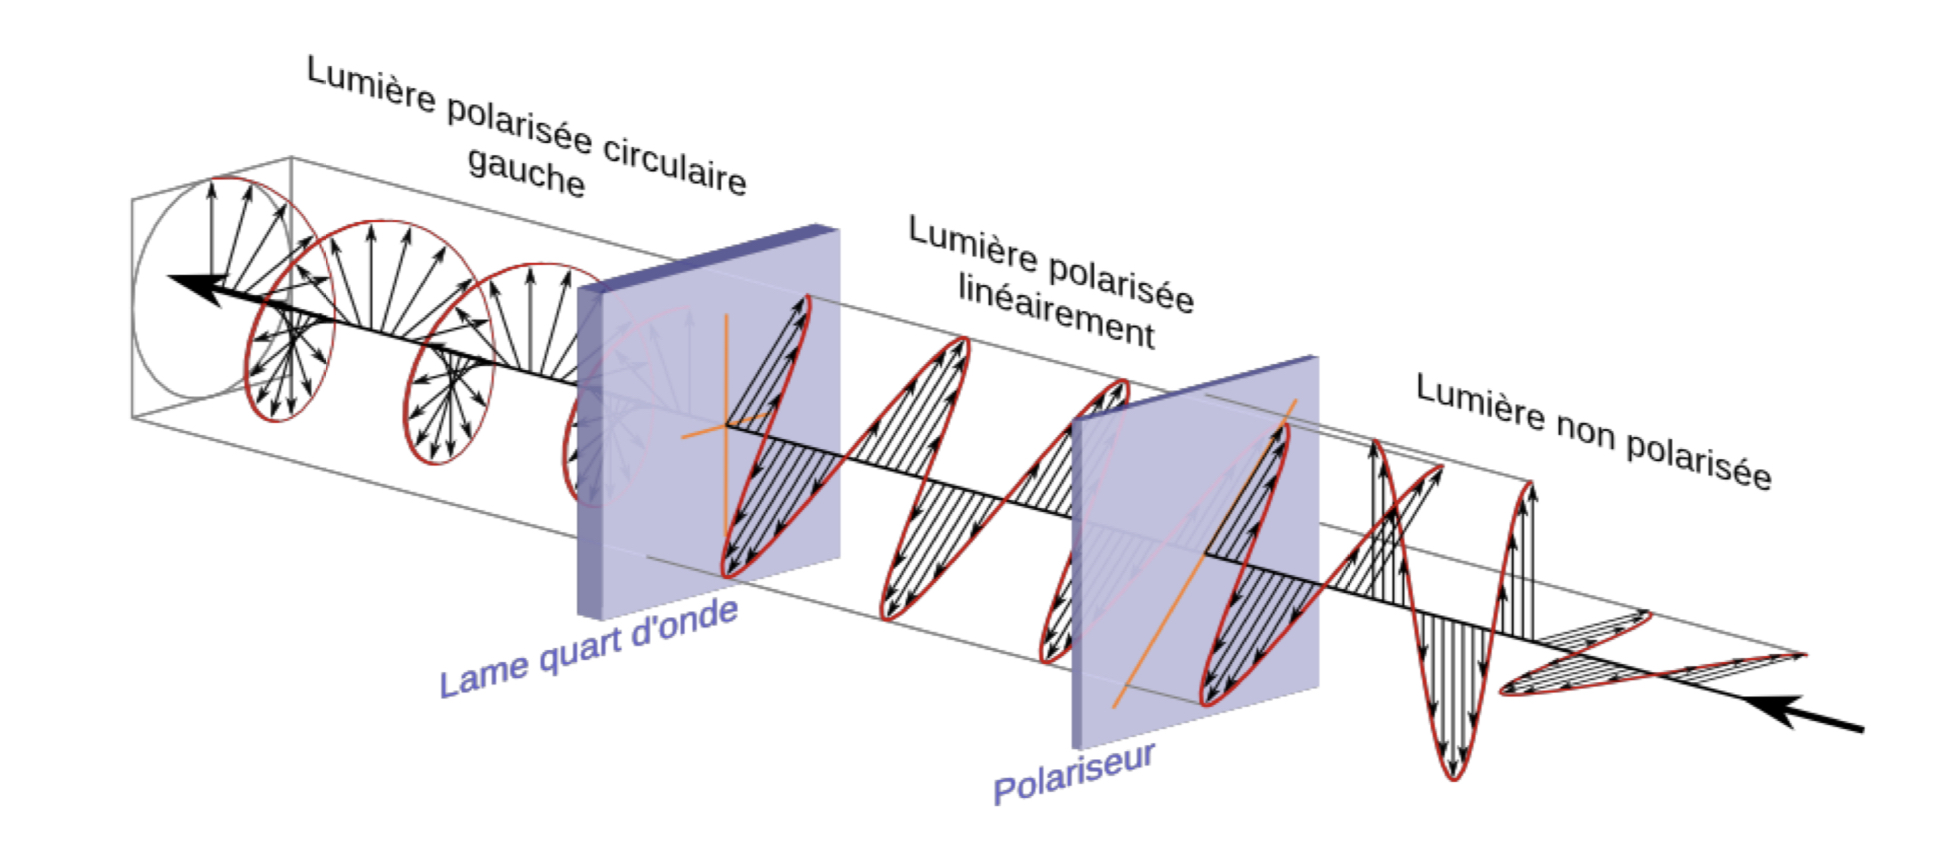
\includegraphics[width=0.8\textwidth]{./assets/PCG.jpeg}
  \caption{PCG}
  \label{fig:PCG}
\end{figure}


\end{Example}






\subsection{Lois de Malus} % (fold)
\label{sub:Lois de Malus}

\begin{Theorem}{Loi de Malus}{}
L'intensité électromagnétique de l'onde transmise est 
\begin{equation}
  I _{ap} = I _{av} \cos ^{2} \alpha
\end{equation}
\end{Theorem}



\newpage

\section{Exercices} % (fold)
\label{sec:Exercices}
\href{https://web.goodnotes.com/s/ICfkODTqFl0XfhFeQCr4Xc}{TD1}
% section Exercices (end)

% subsection Exercices (end)
